%\clearpage
%% -- xsec UL ----------------------
\begin{figure}[h]
  \centering
%    \subfig{0.48}{figures/Result/xsecUL/onestepCC_x12.pdf}{}
%    \subfig{0.48}{figures/Result/xsecUL/onestepCC_varx.pdf}{}
    \subfig{0.48}{figures/Result/xsecUL/symQQC1_x12.pdf}{}
    \subfig{0.48}{figures/Result/xsecUL/symQQC1_varx.pdf}{}
    \subfig{0.48}{figures/Result/xsecUL/symQQC1_dM20.pdf}{}
    \subfig{0.48}{figures/Result/xsecUL/symQQC1_dM30.pdf}{}
    \caption{
    Upper limit of excluded cross-section (95$\%$CL) as the function of the SUSY masses, for the reference model \textbf{QQC1QQC1}, presented in grids (a) $\xhalf$ (b) $\varx$ (c) $\DMtw$ (d) $\DMth$.
    \label{fig::Result::xsecUL::QQC1QQC1} }
\end{figure}

%% --
\begin{figure}[h]
  \centering
    \subfig{0.48}{figures/Result/xsecUL/QQC1BTC1_x12.pdf}{}
    \subfig{0.48}{figures/Result/xsecUL/QQC1BTC1_varx.pdf}{}
    \subfig{0.48}{figures/Result/xsecUL/QQC1BTC1_dM20.pdf}{}
    \subfig{0.48}{figures/Result/xsecUL/QQC1BTC1_dM30.pdf}{}
    \caption{
    Upper limit of excluded cross-section (95$\%$CL) as the function of the SUSY masses, for the reference model \textbf{QQC1BTC1}, presented in grids (a) $\xhalf$ (b) $\varx$ (c) $\DMtw$ (d) $\DMth$.
    \label{fig::Result::xsecUL::QQC1BTC1} }
\end{figure}

%% --
\begin{figure}
  \begin{center}
    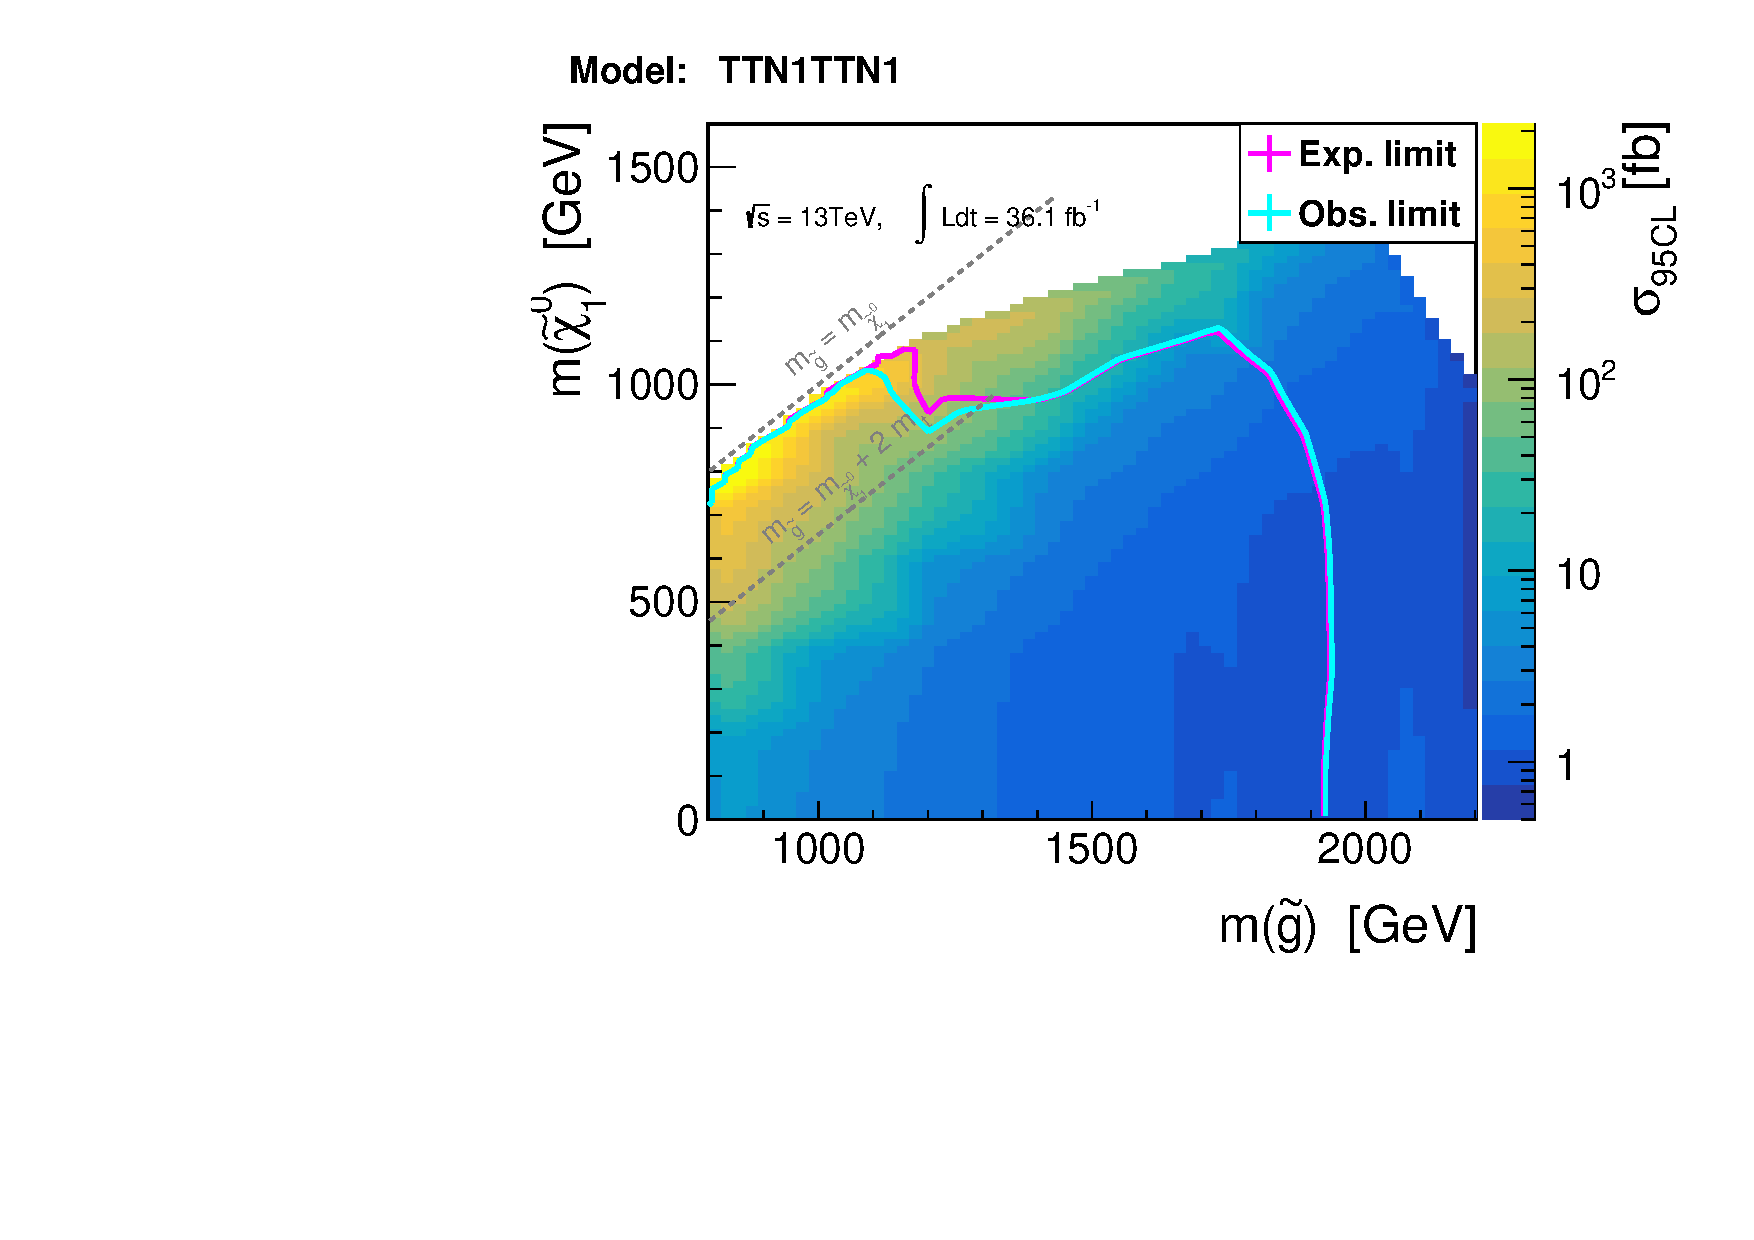
\includegraphics[width=130mm]{figures/Result/xsecUL/symTTN1_x12.pdf}
    \captionof{figure}{
    Upper limit of excluded cross-section (95$\%$CL) as the function of the SUSY masses, for the reference model
 \textbf{TTN1TTN1}.
    \label{fig::Result::xsecUL::TTN1TTN1} }       
  \end{center}
\end{figure}
%-------------------------------                                                                                                   
